\chapter{Market Identification and Sales: Finding Your Customer}

These notes follow Lecture 2 of MIT 15.393, in which Joseph Hadzima handles the course machinery and then turns the room over to Bob Jones for a sustained discussion of finding customers. The curation is by LazyingArt LLC. No validated mathematical frames survive from this lecture, so every displayed relation and every figure below is a cautious reconstruction from the transcript. The lecture's method is itself part of the lesson: begin with a case so simple that we are tempted to dismiss it, and then keep asking the next honest question until the real business either comes into focus or falls apart.

\section{Logistics, Teams, and the Hand-Off to Customer-Finding}

The lecture opens with logistics, but the logistics are already saying something entrepreneurial. Hadzima speaks about attendance, the written requirement, and the preference that the work be done in teams. One reason is comic and administrative: fewer separate submissions are easier to review. The serious reason is the one the lecture wants us to keep. Teams, he says, have a higher probability of success than sole entrepreneurs, which we may summarize as
\begin{equation}
\Pr(\text{success}\mid \text{team})>\Pr(\text{success}\mid \text{solo}).
\end{equation}
That inequality is a compact formalization of a spoken claim, not a theorem proved in the room; but it is the first practical relation of the evening, and it explains why the lecture begins with team formation rather than with product genius.

Only after the course structure is in place does Hadzima hand the room to Bob Jones. Jones immediately makes a contract with the audience. If he is going to ask for ninety minutes of attention, he says, he ought to return something worthwhile for that investment. He therefore asks two questions before he teaches anything substantive: who are you, and what do you want? The room turns out to be mixed. Some people are already on a second venture, some are in their first, some are seriously considering one after graduation, and some are simply exploring. The jokes matter here: medication is available for first-time founders; exploratory work can be as unacademic and as useful as springboard diving during IAP. The room is heterogeneous, and Jones wants the argument to be usable across that range.

This is why he makes his anti-academic turn. He mocks the sort of lecture that begins with a sentence about risk aversion, mean-variance utility maximization, and quadratic utility functions, gets dutifully written down, and leaves nobody any wiser. That joke is not the content of the lecture. It is the permission for the method. Jones tells us he will go in the opposite direction: start with examples so simple they are almost trivial, and let the complexity arrive only when the example itself demands it. That is the pedagogical pivot on which the whole chapter turns.

\section{Start at the End: Money Needed, Customer Value, Customer Count}

Jones now gives us the toy model. Suppose, he says, that he flees the overcharged intellectual world, moves to the Berkshires, becomes a grumpy old man in a tiny house, and decides to give guitar lessons. He can imagine the whole thing very easily: beginner chords, tuning, groove, rhythm, more advanced work, even how to play a mixolydian solo that still sounds like the blues. He would need a small studio, a few amplifiers, perhaps a drum machine. Then he stops himself: let us stop right there.

\subsection{Question \& Answer}

What mistake did he make? The answer is the first conceptual obstacle of the lecture. We are often quick to ask whether we \emph{could} do a venture. Jones insists that we must first ask whether we \emph{should} do it. The bridge from the first question to the second is money. Most companies die, he says, because they run out of money or because they are on a path where they will never make any.

So he reverses direction and begins at the end of the story. We want to make enough money. That means we need revenues, and those revenues should exceed our costs:
\begin{equation}
R>C.
\end{equation}
Revenues come from customers. So the real problem is not ``I have a product idea'' but ``how many customers do I need, and is that number sane?''

The notation here is a cleaned reconstruction of Jones's spoken arithmetic, not notation visibly written in the room. Let \(M\) denote the amount of money we need over a chosen period, and let \(V_c\) denote the value of one customer over that same period. Then the required customer count is
\begin{equation}
N=\frac{M}{V_c}.
\end{equation}
In this lecture \(V_c\) is not a grand lifetime-value formula. It is simply what one active customer is worth on the same monthly or yearly clock used for \(M\).

Jones gives the numerical skeleton in one line:
\begin{equation}
\frac{1{,}000{,}000}{1{,}000}=1{,}000.
\end{equation}
If we need a million dollars and each customer is worth a thousand, then we need a thousand customers. Only after that division do we ask the practical question: how are we going to do that?

\begin{figure}
\centering
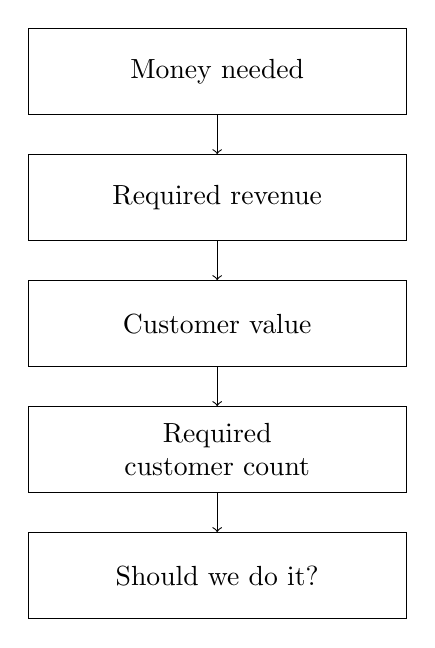
\begin{tikzpicture}[x=1cm,y=1cm]
\draw (0,0) rectangle (4.8,1.1);
\draw (0,-1.6) rectangle (4.8,-0.5);
\draw (0,-3.2) rectangle (4.8,-2.1);
\draw (0,-4.8) rectangle (4.8,-3.7);
\draw (0,-6.4) rectangle (4.8,-5.3);

\node[align=center] at (2.4,0.55) {Money needed};
\node[align=center] at (2.4,-1.05) {Required revenue};
\node[align=center] at (2.4,-2.65) {Customer value};
\node[align=center] at (2.4,-4.25) {Required\\customer count};
\node[align=center] at (2.4,-5.85) {Should we do it?};

\draw[->] (2.4,0) -- (2.4,-0.5);
\draw[->] (2.4,-1.6) -- (2.4,-2.1);
\draw[->] (2.4,-3.2) -- (2.4,-3.7);
\draw[->] (2.4,-4.8) -- (2.4,-5.3);
\end{tikzpicture}
\caption{Transcript-derived reconstruction of Jones's backward logic. We do not start from enthusiasm for the offering; we start from the money requirement and work backward until the venture either looks feasible or does not.}
\end{figure}

Now the toy business is run through the arithmetic. Jones wants only a modest living. On a monthly time base,
\begin{align}
M &= \$5{,}000/\text{month},\\
V_c &= 25\ \$/\text{hour}\times 2\ \text{sessions/month}
     = 50\ \$/\text{customer/month},\\
N &= \frac{M}{V_c}
   = \frac{5{,}000}{50}
   = 100.
\end{align}
A hundred customers is not frightening for a large organization. It is a very different number for one grumpy guitarist starting alone. Jones does not hide that discouraging answer. The arithmetic is supposed to hurt a little. That pain is the point. It is cheaper to discover the problem in five lines of arithmetic than in two years of effort and most of a life savings.

\section{Users, Payers, Champions, and What We Are Really Selling}

Having forced the first go/no-go calculation, Jones now asks the question he had postponed: what exactly is broken here, and who pays us to fix it? The default answer is schoolchildren. They are the obvious users. But they are not the obvious buyers. Past a certain point, Jones says quite plainly, the users are not the customers. The parents are the ones who pay. Once we notice that, the economics remain the same but the meaning changes. The child may want fun, status, escape from boredom, or maybe music itself. The parent may be buying activity, discipline, social development, or merely an experiment.

The lecture then performs its first major reset. Jones says, in effect, erase that and start over. What if the relevant customer is not the child but the adult who used to play, used to sing, used to feel cool, and misses all of that? He gives a much richer version of the service: teach a recognizable tune on Tuesday, assemble an ensemble, and let the person play it with others on Thursday. The ticket is no longer mere instruction. It is competence regained, identity recovered, and performance made possible. The arithmetic shifts with it:
\begin{align}
V_c &\approx 50\ \$/\text{hour}\times 2\ \text{sessions/week}\times 4\ \text{weeks/month}\\
&\approx 400\ \$/\text{customer/month},\\
N &\approx \frac{5{,}000}{400}=12.5.
\end{align}
Jones rounds the answer in words: about a dozen or so.

He pushes the point once more with the older adults he has seen through volunteer music work. Here the same visible format meets yet another need: social life, purpose, companionship, getting out of the house, perhaps even the possibility of romance. The lesson is not that one should randomly mutate the market. It is that changing the customer definition changes the economics because it changes the benefit being purchased.

\begin{table}
\centering
\begin{tabular}{|p{0.28\linewidth}|p{0.20\linewidth}|p{0.22\linewidth}|p{0.16\linewidth}|}
\hline
Customer definition & Primary payer & Approx.\ customer value per month & Customers needed for \(\$5{,}000/\text{month}\) \\
\hline
Schoolchildren taking lessons & Parents & \(\$50\) & \(100\) \\
\hline
Lapsed adults wanting to play again & Adult learner & \(\approx \$400\) & \(\approx 12.5\) \\
\hline
Older adults seeking music and company & Adult learner & \(\approx \$400\) & about a dozen \\
\hline
\end{tabular}
\caption{Transcript-derived comparison of three customer definitions for roughly the same underlying teaching activity. The lesson is that the economics change when the payer and the perceived benefit change.}
\end{table}

\subsection{Question \& Answer}

Who wins if I win? Jones slows the room down over this question because it widens the frame. The first answer is customers, and that answer is correct but incomplete. Customers may become a sales force by talking to one another. End users may become champions. Economic buyers may not be the same people as the users. Adjacent businesses may benefit from our success.

His music-store example is the cleanest illustration. A lapsed guitarist goes into a shop to buy strings, stares at the instruments on the wall, and explains that he has lost his chops and has no real setting in which to play. The helpful person in the store says, in effect, I know a guy who can fix that. If the customer starts taking lessons, the store may later sell strings, better instruments, and more equipment. We win; the store wins; the player wins. This is not generic referral marketing. It is a structural point about aligned incentives.

At this stage Jones asks the other crucial question: what are we really selling? One student says romance. Jones half laughs, half accepts, and then clarifies. We are selling comfort, socialization, purpose, collaboration, and the excitement that comes when ensemble performance suddenly clicks. The anecdote about Jones himself walking into a blues jam, playing with strangers, and feeling ``magic'' happen is not decoration. It is a phenomenology of the benefit. The guitar lesson is the visible product. The invisible product is the life the customer gets to step back into.

\section{The Non-Negotiable Requirement: Customers}

Having extracted a surprising amount from a tiny guitar business, Jones tightens the screws. He now lists the venture questions in a blunter form. We should ask:
\begin{enumerate}
\item What is broken?
\item Who specifically wants a solution?
\item Are there enough of those people?
\item Will they spend money to solve the problem?
\item How are they solving it now?
\item Why is our answer compellingly better than the alternatives?
\item Who actually pays?
\item How do we find them and let them know about us?
\end{enumerate}
The questions are easy, he says. The answers are not. But if we do not at least face these questions, we will drive straight into the hole and only discover it when it is too late.

This is also the moment where the lecture pivots toward investor logic. Jones repeats Hadzima's hard framing: most investors lose most of their money. He jokes that perhaps only eight out of ten fail at MIT instead of nine out of ten elsewhere, but the odds are still dreadful. So the investor wants the answer to two questions: how will you make money, and how will I make money? The order matters. If the venture cannot answer the first question, there is no point even asking the second.

From that perspective, there is only one non-negotiable requirement. We must have customers. Everything else can be renegotiated. Jones says this with the force of a room trying to get away with something and being told that it cannot. We do not have to be rich. We do not have to be beautiful. We do not even have to look especially brilliant. If we have customers, the rest of the world begins to reinterpret us. That is the bridge into the first serious case study. Enough of the abstract, he says. Here is what it looks like when smart people get this wrong.

\section{Customer Discovery by Failure: The Regain Case}

The first medical case arrives only after the scaffold is in place, and the sequencing matters. Jones wants us to hear how reasonable a bad plan can sound. He was running the clinical nutrition division of a medical company in California, a division whose economics were excellent:
\begin{equation}
\text{cost per liter}\approx \$3,
\qquad
\text{sale price per liter}\approx \$70.
\end{equation}
The broader company had been doing roughly two hundred million dollars a year for a long time, but managed care threatened the old profit pool. So Jones went looking for the next revenue source and found, as he says, an opportunity nobody else was pursuing. He immediately adds the correct diagnosis in hindsight: that should have been a red flag.

The field was kidney dialysis. The background numbers looked attractive:
\begin{equation}
400{,}000\ \text{patients},
\qquad
2{,}300\ \text{dialysis centers},
\qquad
8\text{--}12\ \text{lb fluid gain between treatments}.
\end{equation}
The contradiction also looked obvious. Dialysis patients often need nutritional supplementation, but the standard supplements were liquids, precisely the thing these patients should not be loading up on. So the company designed a bar-like product, high in what patients needed, low in what they should avoid, and without added fluid. The product was named \emph{Regain}.

The company did the respectable things. It ran a clinical trial even though it was not required. It published the result. The result was good: blood chemistries improved, lives were extended. It then asked opinion leaders, clinicians, and dieticians whether they would recommend the product. The answer, extraordinarily, was yes. For how many patients? All of them. How often? Seven days a week. At what price? Roughly \(\$3\) per bar. The arithmetic looked almost too good. Jones says they began to think they had replaced the business they were afraid of losing.

Then the product was launched, and the floor dropped out:
\begin{equation}
\$400{,}000\ \text{forecast}
\qquad \text{versus} \qquad
\$35{,}000\ \text{actual}.
\end{equation}
As a cleaned-up ratio,
\begin{equation}
\frac{35{,}000}{400{,}000}=0.0875<0.10.
\end{equation}
Month after month, the product came in at less than ten percent of forecast.

\subsection{Question \& Answer}

What did we do wrong? Jones lets the question sit in the room because the answer comes in layers.

\begin{enumerate}
\item We interviewed clinicians, but the patients were the buyers.
\item We judged taste with the wrong palate.
\item We mistook clinical need for willingness to pay.
\item We misunderstood the motivational composition of the market.
\item We forgot that retailers were customers too.
\end{enumerate}

The first two mistakes are concrete. Clinicians did not buy the product and did not eat it. Patients did both. When Jones's team finally spoke to patients, they learned that many did not want the product and could not afford it. The taste problem was equally sobering. In kidney failure the palate shifts, and a heavily protein-based product can taste like spoiled meat. The team had asked the wrong people how it tasted.

The third and fourth mistakes cut deeper. Jones says the real question should have been: who gets kidney failure? The transcript gives a rough decomposition,
\begin{equation}
33\%+44\%=77\%\approx \frac{3}{4},
\end{equation}
which he interprets as follows: about three quarters of the customer base had arrived there through long-term mismanagement of diabetes or high blood pressure. His conclusion is brutal but plain. A great many of these patients had not taken care of themselves before. Many were not going to start now. Clinical benefit was real, but motivation to spend was weak.

The final mistake is the one the lecture keeps widening toward. Patients still had to buy the product somewhere. Jones's company understood hospitals; it did not understand retail pharmacy. That ignorance was expensive. A pharmacy manager has only seconds to hear a pitch. A shelf is a monetized asset. Remove a known product, insert an unknown one, and the retailer wants compensation. That is the logic of slotting fees, and Jones gives the number that made the lesson unforgettable:
\begin{equation}
\$1{,}000{,}000\ \text{per quarter for CVS},
\end{equation}
before guaranteed sales, refunds, and chain-wide stocking requirements were even fully counted.

The failure therefore was not one error but a stack of errors, each caused by a different bad definition of customer. Jones later found a way to reach the roughly twenty-five percent of the market that had not arrived through self-neglect, and the broader company recovered. But the lesson of the year is not rescue. It is diagnosis. The consequences of not thinking through the customer system got worse and worse.

\section{Rebuilding the Business Around the Real Customer: Nighttime Diabetes}

With characteristic dark humor, Jones says that entrepreneurship may be a form of mental illness, because after all this he went off and did more of it. The next medically grounded venture is the constructive answer to the Regain failure. This time the company enters diabetes, and the starting point is not a product gap but a lived problem.

The market is large:
\begin{equation}
10{,}000{,}000\ \text{diagnosed patients},
\qquad
4{,}000{,}000\ \text{insulin users}.
\end{equation}
The practical aim of diabetes management, as Jones states it, is to keep blood glucose from fluctuating wildly. If we denote the overnight glucose level only schematically by \(g(t)\), then we should read the next picture as a qualitative shape, not as a clinical graph with calibrated axes. During the day, disciplined patients can spread intake and insulin across small meals and small snacks. At night that discipline is much harder to sustain. Instead people tend to eat a large bedtime snack, take a large insulin bolus, and hope the two will titrate through the night.

The hope fails for a simple reason. The food turns to glucose quickly. The spike is higher, but the support does not last longer. Jones identifies the dangerous interval as
\begin{equation}
2\ \text{a.m.}\le t\le 6\ \text{a.m.},
\end{equation}
the period in which food support has run out but insulin may still be working.

\begin{figure}
\centering
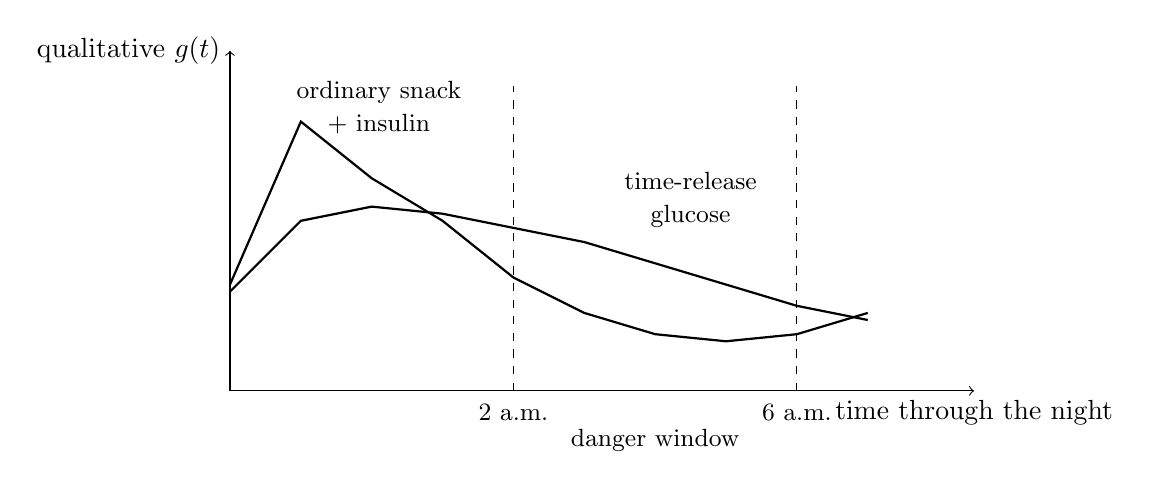
\begin{tikzpicture}[x=0.9cm,y=0.09cm]
\draw[->] (0,0) -- (10.5,0) node[below] {time through the night};
\draw[->] (0,0) -- (0,48) node[left] {qualitative \(g(t)\)};

\draw[dashed] (4,0) -- (4,43);
\draw[dashed] (8,0) -- (8,43);
\node at (4,-3) {\small 2 a.m.};
\node at (8,-3) {\small 6 a.m.};
\node at (6,-7) {\small danger window};

\draw[thick] plot coordinates {(0,15) (1,38) (2,30) (3,24) (4,16) (5,11) (6,8) (7,7) (8,8) (9,11)};
\draw[thick] plot coordinates {(0,14) (1,24) (2,26) (3,25) (4,23) (5,21) (6,18) (7,15) (8,12) (9,10)};

\node[align=center] at (2.1,40) {\small ordinary snack\\\small + insulin};
\node[align=center] at (6.5,27) {\small time-release\\\small glucose};
\end{tikzpicture}
\caption{Transcript-derived schematic of the overnight problem. The ordinary bedtime snack gives a sharper early spike without widening the safe interval, whereas the redesigned product is meant to spread glucose availability further into the night.}
\end{figure}

At this point the lecture changes pace. Jones explains focus groups, then rebels against the standard focus-group script. After too much science and too much intellectual talk, he bursts out and asks what the customers are actually afraid of. The answer is the first true emotional discovery of the case: some people no longer sleep in a bed because they are afraid they will get too comfortable and die in their sleep. That is the sentence around which the business is rebuilt.

So the company creates a product whose components convert to glucose at different rates and last all night. Jones says that, being marketers at heart, they called it time-release glucose. Later in the lecture he refers to the resulting business by product name, \emph{Night Bite}. This time, he adds pointedly, it also tasted good.

\subsection{Question \& Answer}

Why would putting ``for diabetes'' on the label kill the business? Jones raises this as a genuine puzzle because he originally fought to be able to say exactly that on the package. The customers corrected him. It is nobody's business, they say, that I have diabetes. I am not ``a diabetic'' in the public sense; I am a banker, a lawyer, an entrepreneur, an active professional. If I pull out something that looks like medicine during a meeting, people will think I am sick, frail, and professionally diminished. That is a career-limiting signal.

So the product has to look like something an elite athlete might use, not like medication. The chemistry can be medical; the public identity cannot. That is why the company gives it a non-medical name and why Jones later notes, with some satisfaction, that marathon runners ended up buying it too.

The redesign also becomes more precise because the company now talks not only to clinicians but to parents and patients. The unit is made deliberately small and divisible:
\begin{equation}
100\ \text{calories per unit},
\end{equation}
with scored use that allows \(50\), \(100\), or \(150\) calories depending on the user. A better product has now emerged. But Jones is careful not to stop there. A better product is still only half a business. The next problem is distribution.

\section{Channels, Free Sales Forces, and Selling Customers to Retailers}

Jones now slows the story down and turns to what he calls the nuts and bolts. The first discovery is that channel changes perceived value. In a focus group the company puts paper in front of users and asks two questions: where would you expect to buy a product like this, and how much would you expect to pay? The answers sort into two piles:
\begin{equation}
\$0.49 \text{ in a grocery store},
\qquad
\$1.25 \text{ in a pharmacy.}
\end{equation}
Same product, different channel, different value. Jones says, dryly, call me silly, I like pharmacies.

The next discovery is organizational. A business like this does not sell to ``the market'' in one undifferentiated move. It sells through a customer system. The crucial intermediary turns out to be the certified diabetes educator. These professionals can literally be found by zip code through their association. More importantly, they have a professional frustration: patient compliance. They tell patients what to do, and the patients do not do it. If Jones can give them something patients will actually use and thank them for recommending, he has found people who win if he wins.

\begin{figure}
\centering
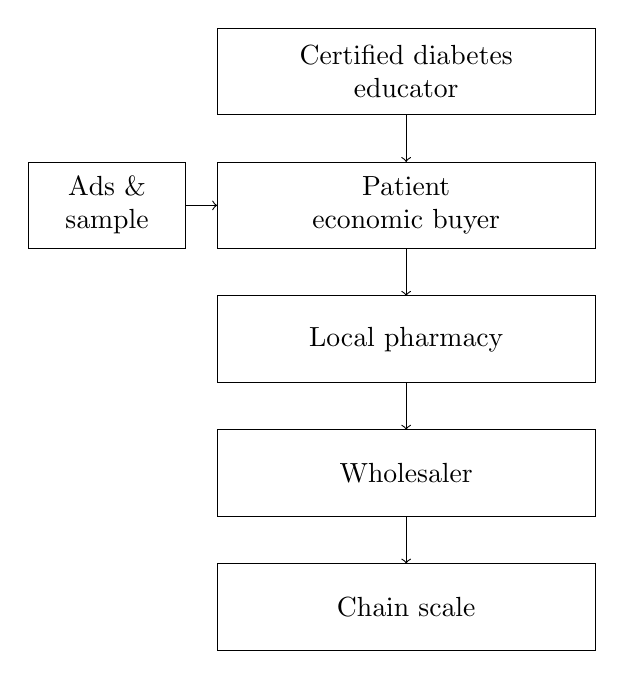
\begin{tikzpicture}[x=1cm,y=1cm]
\draw (0,0) rectangle (4.8,1.1);
\draw (0,-1.7) rectangle (4.8,-0.6);
\draw (0,-3.4) rectangle (4.8,-2.3);
\draw (0,-5.1) rectangle (4.8,-4.0);
\draw (0,-6.8) rectangle (4.8,-5.7);

\draw (-2.4,-1.7) rectangle (-0.4,-0.6);

\node[align=center] at (2.4,0.55) {Certified diabetes\\educator};
\node[align=center] at (2.4,-1.15) {Patient\\economic buyer};
\node[align=center] at (2.4,-2.85) {Local pharmacy};
\node[align=center] at (2.4,-4.55) {Wholesaler};
\node[align=center] at (2.4,-6.25) {Chain scale};
\node[align=center] at (-1.4,-1.15) {Ads \&\\sample};

\draw[->] (2.4,0) -- (2.4,-0.6);
\draw[->] (2.4,-1.7) -- (2.4,-2.3);
\draw[->] (2.4,-3.4) -- (2.4,-4.0);
\draw[->] (2.4,-5.1) -- (2.4,-5.7);
\draw[->] (-0.4,-1.15) -- (0,-1.15);
\end{tikzpicture}
\caption{Transcript-derived reconstruction of the Night Bite customer system. The patient is the economic buyer, but the educator, the pharmacy, and the wholesaler each carry distinct incentives. The venture only scales when those roles are aligned rather than collapsed into one vague ``customer.''}
\end{figure}

Several thousand educators eventually become a kind of unpaid sales force. Jones is careful about why. They are not unpaid because they are fools; they are unpaid because they are healers, and what they want is not commission but something their patients will comply with. The educators can then recommend the product to patients and even help pressure local pharmacies to stock it.

The company first sells directly, not because that is the intended endpoint but because Jones wants information. He wants reorder frequency so he can infer usage. Advertising generates inbound calls, and the numbers become a kind of live demand function:
\begin{equation}
100,\ 200,\ 300,\ 500\ \text{calls/day}.
\end{equation}
At the same time, long-run usage turns out to be strikingly strong:
\begin{equation}
\text{reuse rate}>300\ \text{occasions/year}.
\end{equation}
That is not a market-research fantasy. It is behavioral evidence.

Jones also gives a small methodological lesson from inside sales. Closed-ended questions stop the conversation too quickly. ``Did you like it?'' can end with ``no.'' An open-ended question such as ``What did you think?'' keeps the door open long enough to discover that taste may have been imperfect, efficacy was good, and the customer wants to reorder anyway.

The pharmacy-entry tactic is equally concrete. A store manager may have a purchase amount below which corporate approval is unnecessary. Jones guesses that threshold is about one hundred dollars and prices the starter kit just below it:
\begin{equation}
\$99.95<\$100.
\end{equation}
The risk is removed: if it does not sell, throw it away and get a refund. Then the company calls its existing customers and tells them where the product is now stocked. When the first batch sells out, the pharmacy itself becomes interested. The phrase Jones uses is exact and worth preserving: he bought a bunch of customers and then sold those customers to the retailers.

The same logic is pushed upstream. A large pharmacy may carry about eight thousand SKUs and does not want eight thousand invoices. So the company gets into wholesalers by seeding nearby pharmacies, giving the wholesaler its normal margin, and asking only to be entered into the system before reorder demand appears. Once that is done, scale becomes possible.

The planogram meeting at a major chain is the final demonstration. Jones and his colleague go into a fifteen-minute meeting with no money to pay slotting fees. They spend ten minutes saying who they are and why the product is good, and then open a briefcase full of printouts showing ten thousand existing diabetes customers in the states where the chain operates. Those customers all have one question: which pharmacy carries the product? How, they ask the buyer, would you like us to answer them? Jones then says nothing. He invokes the negotiating rule of thumb that the next person who speaks loses. After the silence, the buyer says yes. What won the meeting was not persuasion in the abstract. It was customers.

\section{Segment by Motivation, Not Demographics}

By the end of the Night Bite story the lecture has earned the right to become doctrinal. Jones turns back to the room and asks what he should have learned from all these experiences.

\subsection{Question \& Answer}

The audience answers, and Jones sharpens the answers as he goes. The resulting principles are the real retrospective of the lecture:
\begin{enumerate}
\item Talk to your customers.
\item Let the customer definition evolve as the business evolves.
\item Reinvest early effort and money in better market knowledge.
\item Treat distribution as part of the venture, not as an afterthought.
\item Figure out what people are really buying.
\end{enumerate}

That last point becomes a short theory of benefits. Nobody specifically wants the product. People want what the product does. Jones's example is vision: we may hire glasses, contact lenses, or a LASIK surgeon, but what we really want is to see better. The same principle reaches backward through the entire lecture. Nobody wanted ``guitar lessons'' in the narrow sense. They wanted social life, competence, romance, purpose, performance, collaboration. Nobody wanted ``glucose'' in the narrow sense. They wanted safety, sleep, and the ability to function without public stigma.

Jones then asks what market segmentation really means. Conventional marketers segment by geography, income, or gender. He argues that the entrepreneur, especially the undercapitalized entrepreneur, must segment by motivation. The transcript's cleanest example is the product that prevents a second heart attack. The person who has just survived the first one sits at the top of the motivation pile. Nearby family members may listen next. Social peers may pay some attention after that. The broad public is the low-motivation block at the bottom:
\begin{equation}
\text{most motivated}
>
\text{related observers}
>
\text{adjacent social group}
>
\text{general public}.
\end{equation}
That ordering is qualitative, not measured. Its meaning is strategic. A startup cannot afford to spend scarce resources trying to convert the least motivated part of the world. Jones calls that big bottom block a graveyard.

The comparison between Regain and Night Bite makes the principle vivid. Regain improved clinical markers, but the patient felt no immediate difference. Every six months the doctor might say, nice going, your blood chemistries are better. Night Bite produced immediate morning feedback: I think it worked. In Jones's joking form, the user did not wake up dead. The line is facetious, but the point is exact. Motivation rises when the benefit is not only real but felt.

He then compresses his own view of marketing almost to absurdity. After acknowledging all the sophisticated mechanics, he says he can save us two years of graduate school with two bullet points, and the two bullet points are the same: find out what your customers want; then find out what your customers want. The repetition is not carelessness. It is emphasis.

The very last quick story before the closing homework lands the lesson one final time. Jones says a group of them once invented a sleep-support product and, in a foolish top-down move, decided the market was working moms. They assembled a huge list. They heard nothing. Then a few repeat purchasers emerged, and when Jones called them personally and asked why they were buying, every answer turned out to be some version of the same thing: I run marathons, I need better recovery, better sleep helps me recover, and therefore your product helps me perform. Jones thought he was selling sensitivity and care. He was selling to warriors. He says flatly that he would have died of old age before learning that from a sequence of Google ads. Talk to them.

That is why the lecture ends by narrowing, not widening. The next session will be about pitching. The homework is to pitch the business in three minutes, then in thirty seconds, then, if possible, in three sentences and about ten seconds. The compression is not a new topic. It is the compressed form of everything in this lecture.

\section{Summary}

The lecture begins with attendance codes and team formation, but its real structure is mathematical and strategic. We begin at the end of the story, ask how much money we need, estimate what one customer is worth, and derive how many customers are required. Then we ask the harder questions: who is the user, who is the payer, who is the champion, who else wins if we win, and what benefit is actually being purchased?

The Regain case shows how completely a business can fail even when the clinical result is real and the arithmetic looks encouraging. The Night Bite case shows how the same kind of medically grounded business can succeed once fear, identity, channel, and reorder behavior are taken seriously. The final principle is severe and practical: do not aim at everybody. Find the people who want the offering most, learn what they are really buying, and build the venture around them.